\section*{Problem 6}

The model is $\dot x=\nu\cos\theta$, $\dot y=\nu\sin\theta$, $\dot\theta=\omega$, $\dot\nu=u_1$, $\dot\omega=u_2$, with $V=\mathbf{x}^T\mathbf{x}$ where $\mathbf{x}=[x,y,\theta,\nu,\omega]^T$.

\subsection*{1. Derivative of $V$}

\[
\dot V=2\mathbf{x}^T\dot{\mathbf{x}}
=2\big[x\nu\cos\theta+y\nu\sin\theta+\theta\omega+\nu u_1+\omega u_2\big].
\]

\subsection*{2. The given control law}

Putting in $u_1=-k_1\nu-x\cos\theta-y\sin\theta$ and $u_2=-k_2\omega-\theta$:
\[
\nu u_1=-k_1\nu^2-x\nu\cos\theta-y\nu\sin\theta,\qquad \omega u_2=-k_2\omega^2-\theta\omega ,
\]
so the cross terms cancel and
\[
\dot V=-2k_1\nu^2-2k_2\omega^2\le0 .
\]
$V$ is positive definite and radially unbounded, so the origin is stable and trajectories stay bounded. But $\dot V$ is only negative semidefinite (it is zero whenever $\nu=\omega=0$), so this does not give asymptotic stability. I used LaSalle.

On $\{\dot V=0\}=\{\nu=\omega=0\}$, staying there requires $\dot\omega=u_2=-\theta=0$, so $\theta\equiv0$, and $\dot\nu=u_1=-x\cos\theta-y\sin\theta=-x=0$, so $x\equiv0$. Nothing forces $y$ to zero, so the largest invariant set is
\[
\mathcal M=\{(0,\,y,\,0,\,0,\,0):\ y\in\mathbb R\}.
\]
Every point in $\mathcal M$ is an equilibrium of the closed loop, so trajectories converge to \emph{some} point on that line but not necessarily the origin.

\textbf{Conclusion: this controller does not asymptotically stabilize the origin.}

\emph{Quantitative.} The equilibrium set is a whole line, so the origin is not isolated and cannot be asymptotically stable. Linearizing the closed loop at $0$ gives $\ddot x=-k_1\dot x-x$, $\ddot\theta=-k_2\dot\theta-\theta$ and $\dot y\approx0$, so the eigenvalues are the roots of $s^2+k_1s+1$, $s^2+k_2s+1$ and an extra $s=0$ from $y$. In simulation with $k_1=k_2=1$ (Fig.~\ref{fig:p6}) the states $x,\theta,\nu,\omega$ all go to zero but $y$ ends at $0.664$, $-0.949$ and $1.435$ for the three initial conditions I tried, and $V$ decreases but does not reach zero.

\emph{Qualitative.} The robot cannot move sideways, so $y$ only changes when $\nu\sin\theta\neq0$. The controller drives $\theta$ and $\nu$ to zero, which freezes $y$ wherever it happens to be. This is the usual nonholonomic problem: no smooth static feedback can asymptotically stabilize this kind of system (Brockett), so you need something time-varying or discontinuous.

\begin{lstlisting}
Vdot = simplify(expand(2*q.'*f_cl));      % -2*k1*nu^2 - 2*k2*om^2
[t, S] = ode45(dyn, [0 200], inits{i}, opts);
\end{lstlisting}

\begin{figure}[h]
\centering
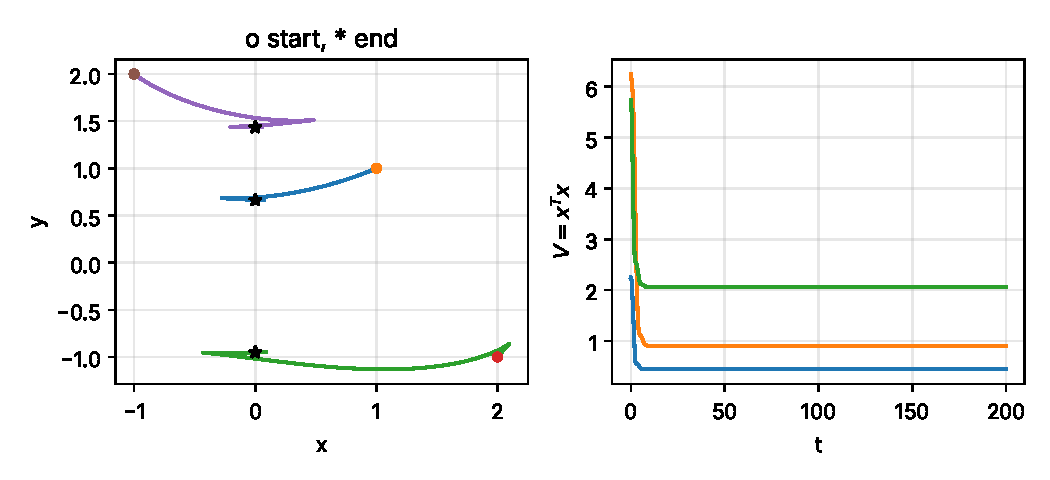
\includegraphics[width=0.85\linewidth]{figures/p6.pdf}
\caption{Closed-loop trajectories end on the line $x=\theta=0$ at $y\neq0$ (left); $V$ does not go to zero (right).}
\label{fig:p6}
\end{figure}
